\apendice{Especificación de diseño}

\section{Introducción}
En este anexo se explica la estructura del proyecto, tanto de archivos como de datos.\\
Se realizan gráficos para que visualmente resulte más sencillo comprender la estructura.
\section{Diseño de datos}
Para la relización del TFG se ha utilizado un fichero csv y una base de datos.
\subsection{Estructura de la base de datos:}
La base de datos se ha realizado con PostgreSQL y cuenta con tres tablas (Figura C.1):
\begin{enumerate}
    \item \textbf{USUARIOS:}\\
    La tabla Usuarios contiene el usuario y la contraseña encriptada del rol administrador, que se utilizará para entrar en las opciones avanzadas y recopilación de datos.
    Los usuarios que no tengan las credenciales del administrador, solo podrán visualizar en el mapa la geolocalización de los BICs y sus respectivas estadísticas de los datos almacenados en la tabla de tweets\_patrimonios.\\
    En posteriores versiones de esta aplicación, esta tabla podrá contener usuarios con otros roles, además del administrador.
    \item \textbf{LISTADO\_PATRIMONIOS:}\\
    En la tabla Patrimonios se incluyen todos los Bienes de Interés Cultural especificados en el listado proporcionado por los tutores, con un id identificativo.
    \item \textbf{TWEETS\_PATRIMONIOS:}\\
    En la tabla Tweets\_Patrimonios se incluyen, por id, todos los parámetros obtenidos de la API de Twitter, conectándose a la tabla de Listado\_Patrimonios a través del id del Patrimonio. Esta tabla es la más extensa de la base de datos, pues guardará toda la información obtenida.
\end{enumerate}
\begin{figure}[h]
    \centering
    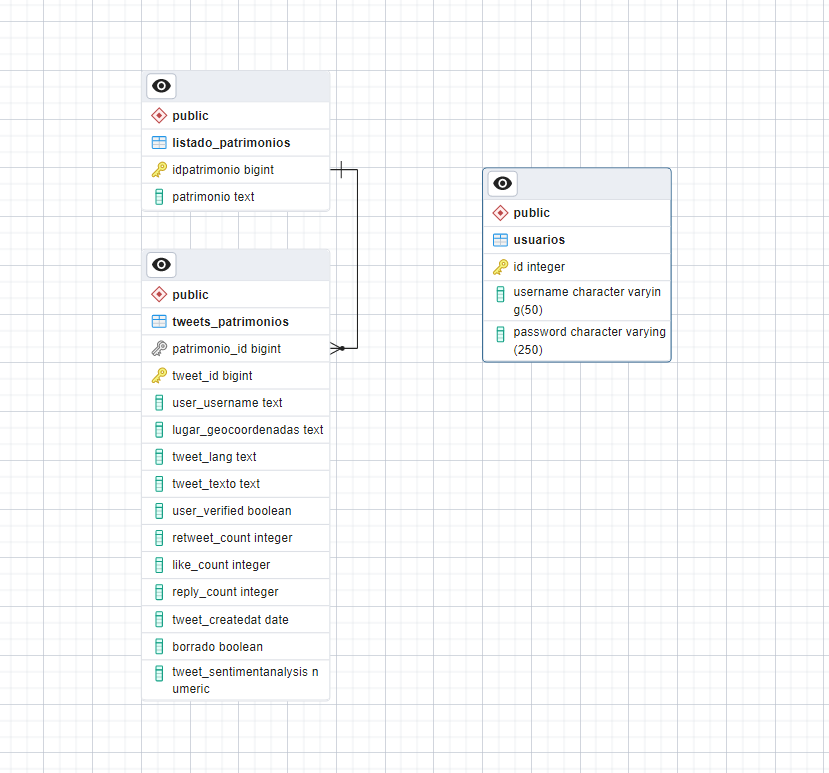
\includegraphics[scale=0.6]{img/TablasBD.PNG} 
    \caption{Diseño de datos - Estructura de base de datos}
     \label{Diseño de datos - Estructura de base de datos}
\end{figure}
Cada una de dichas tablas, a su vez, se descomponen en columnas con la información asociada. La organización que se ha decidido seguir es la siguiente:

\begin{itemize}
    \item \textbf{TABLA USUARIOS:} 
    \begin{enumerate}
        \item Id: número único e identificativo del usuario (en este caso del administrador).
        \item Usuario: usuario con el que se iniciará sesión como 'Administrador'.
        \item Contraseña: contraseña encriptada asociada al rol 'Administrador'.
    \end{enumerate}
    \item \textbf{TABLA LISTADO\_PATRIMONIOS:}  
    \begin{enumerate}
        \item id: número único e identificativo de cada BIC.
        \item Patrimonio: nombre de cada uno de los BICs de la etapa de Castilla y León.
    \end{enumerate}
    \item \textbf{TABLA TWEETS\_PATRIMONIOS:}  
    \begin{enumerate}

        \item Patrimonio\_Id: número único e identificativo de cada BIC que conecta la tabla Tweets\_Patrimonios con esta tabla.
        \item Tweet\_Id: número único e identificativo de cada tweet recopilado.
        \item Lugar\_GeoCoordenadas: identificación del lugar desde donde se publicó el tweet. Puede que no se especifique ubicación en el tweet, por lo que el parámetro se especificará por defecto como "No hay geolocalización".
        \item Tweet\_Lang: idioma en el que se escribe el tweet. Al tratarse de Bienes de Interés Cultural situados en España, se espera que la mayoría de tweets estén en español (es).
        \item Tweet\_Texto: contenido del tweet recopilado de la API.
        \item User\_Username: nombre del usuario que ha publicado el tweet.
        \item User\_Verified: parámetro en el que se indica si el usuario está verificado o no.
        \item Retweet\_Count: parámetro en el que se guarda el número de retweets que ha obtenido ese tweet.
        \item Like\_Count: parámetro en el que se guardará el número de likes que ha obtenido ese tweet.
        \item Reply\_Count: parámetro en el que se guardará el número de respuestas que ha obtenido ese tweet.
        \item Tweet\_CreatedAt: parámetro en el que se especifica la fecha en la que el tweet fue publicado.
        \item Borrado: parámetro no obtenido de la API de Twitter. El administrador, en la creación de la base de datos, especificará la fecha desde la que se requieren los tweets, en caso de que la fecha introducida sea posterior a la primera fecha que consta en la base de datos, los tweets anteriores -y por tanto no requeridos- marcarán este parámetro a 'False' para que en el caso de que después se necesiten no se tengan que realizar tantas consultas a la API y se agilice el proceso de búsqueda.
        \item Tweet\_SentimentAnalysis: valoración numérica entre 0 (negativo) y 1 (positivo) del sentimiento del contenido del tweet calculado con la librería \textit{"sentiment\_analysis\_spanish"}.
    \end{enumerate}
\end{itemize}

\subsection{Estructura de csv:}
El fichero csv ha sido utilizado para obtener parámetros como la localización, destinado al desarrollo del mapa de inicio. \\
Se ha ordenado de tal manera:
\begin{itemize}
   
    \item \textbf{CSV inventario\_01:}  
    En este csv se guarda toda la información recopilada de la Junta de Castilla y León para después hacer uso de ella a la hora de configurar el mapa de la página de inicio de la publicación.\\
    Los parámetros que contiene son: 
    \begin{enumerate}
        \item n: número único e identificativo de cada BIC.
        \item cod\_jcyl: código de ordenación de los BICs para la Junta de Castilla y León.
        \item provincia: provincia a la que pertenece el patrimonio.
        \item municipio: municipio al que pertenece el BIC.
        \item localidad: localidad a la que pertenece el BIC.
        \item denominación: nombre identificativo de cada uno de los BICs.  
        \item categoría: tipo de BIC (castillo, monumento, rollo de justicia...)
        \item latitud: latitud a la que se encuentra el BIC.
        \item longitud: longitud a la que se encuentra el BIC.
        \item altitud: altitud a la que se encuentra el BIC.
    \end{enumerate}
      
\end{itemize}

\section{Diseño procedimental}
En este anexo se muestran los diagramas de secuencia de la aplicación para realizar la explicación del funcionamiento interno de la misma.
\subsection{Visualización de estadísticas}
Se muestra el diagrama de secuencia en la ejecución de mostrar los gráficos estadísticos (Figura C.2).\\

\begin{figure}[h!]
    \centering
    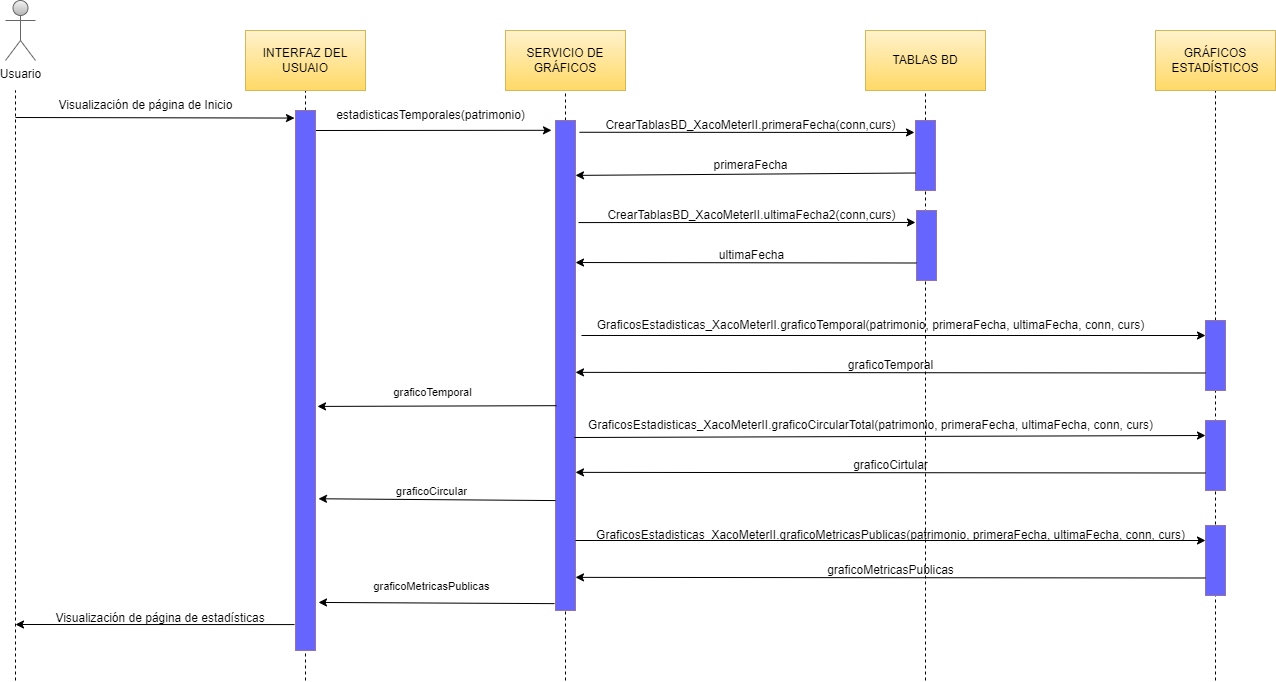
\includegraphics[scale=0.22]{img/DiagramaSecuencias_Estadisticas.png} \\
    \caption{Diagrama de secuencia - Estadísticas temporales}
    \label{Diagrama de secuencia - Estadísticas temporales}
\end{figure}

\subsection{Login}
Se muestra el diagrama de secuencia en la ejecución del inicio de sesión (Figura C.3).\\

\begin{figure}[h!]
    \centering
    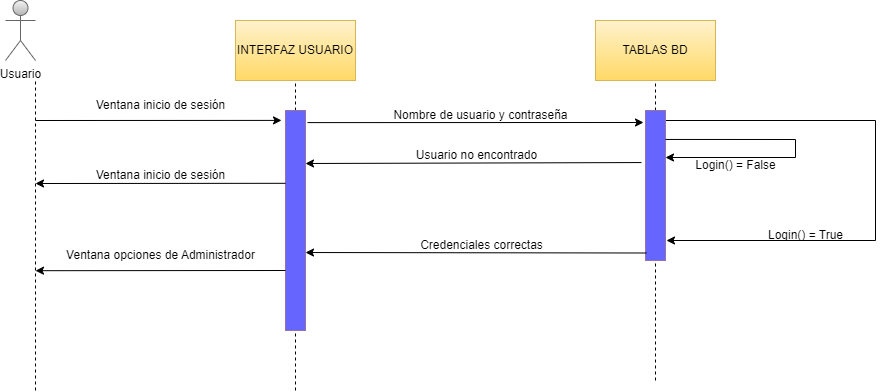
\includegraphics[scale=0.25]{img/DiagramaSecuencias_Login.png}\\
    \caption{Diagrama de secuencia - Inicio de sesión}
    \label{Diagrama de secuencia - Inicio de sesión}
\end{figure}


\subsection{Recopilación de datos}
Se muestra el diagrama de secuencia en la ejecución de recopilación de datos con la API y guardado en la base de datos (Figura C.4).\\


\begin{figure}[h!]
    \centering
    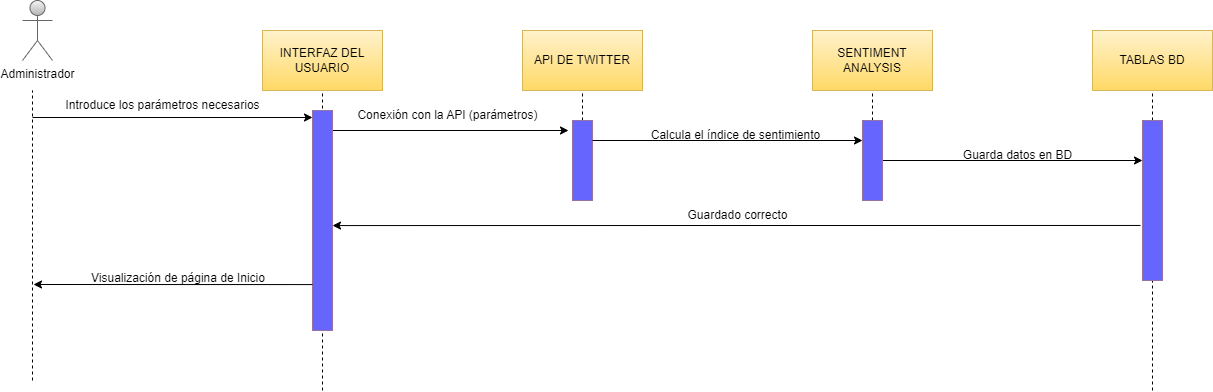
\includegraphics[scale=0.3]{img/DiagramaSecuencias_ActualizarCrear.png} \\
    \caption{Diagrama de secuencia - Creación de datos}
    \label{Diagrama de secuencia - Creación de datos}
\end{figure}



\section{Diseño arquitectónico}
En este apartado se explica el diseño que se ha seguido para desarrollar el proecto, pensado para contribuir a que la aplicación sea fácilmente escalable.


\subsection{Modelo-Vista-Controlador(MVC)}
El diseño Modelo-Vista-Controlador (Figura C.5), como describe su propio nombre, se basa en un patrón con tres componentes:
\begin{enumerate}
    \item \textbf{MODELO:}\\
    Es la lógica de los datos, es decir, el patrón que siguen los datos del programa.\\
    En XacoMeterII, el modelo está compuesto por la base de datos, la estructura del archivo csv y por la lógica que sigue la extracción de los datos de Twitter. 
    
    \item \textbf{VISTA:}\\
    La parte de la vista se refiere a la interfaz gráfica de la aplicación. \\
    En XacoMeterII, la vista está compuesta por todos los archivos \textit{.html} que contiene el proyecto, todos ellos agrupados en el directorio \textit{/templates}.
    
    \item \textbf{CONTROLADOR:}\\
    Es la parte del programa que manda realizar las operaciones, es decir, es el que se encarga de controlar cómo se mandan los datos y como recuperarlos. \\
    En XacoMeterII, el controlador está compuesto por el archivo \textit{main.py}.
    Además, el controlador cuenta con varios servicios que realizan las operaciones más complejas, que en el proyecto son todos los archivos .py incluido en el directorio \textit{/Code}.

\end{enumerate}

\begin{figure}[h!]
    \centering
    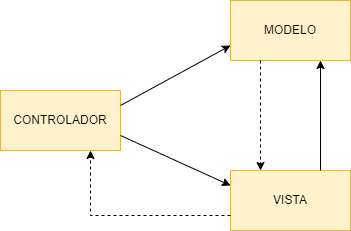
\includegraphics[scale=0.8]{img/MVC.png} \\
    \caption{Diseño arquitectónico - Modelo-Vista-Controlador}
    \label{Diseño arquitectónico - Modelo-Vista-Controlador}
\end{figure}

\subsection{Fachada \textit{(Facade)}}
El patrón fachada o \textit{"Facade"} es un patrón de diseño de software que proporciona una interfaz unificada sencilla que sirve de intermediaria entre los usuarios y el conjunto de interfaces en un subsistema.\cite{fachada}\\
Este patrón (Figura C.6), en este caso, se utiliza para simplificar la interfaz del usuario hacia un subsistema complejo, es decir, los módulos en los que se realizan las operaciones de conexión a la API de Twitter, creación de estadísticas, consultas a la base de datos... \\
En este caso, la fachada es el módulo \textit{main.py}, que comunica todos los módulos con el usuario, siendo así el intermediador.
\begin{figure}[h!]
    \centering
    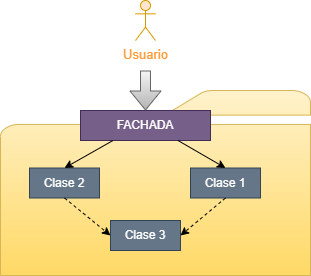
\includegraphics[scale=0.8]{img/patronFachada.png} \\
    \caption{Diseño arquitectónico - Fachada}
    \label{Diseño arquitectónico - Fachada}
\end{figure}
